\documentclass[aspectratio=169]{beamer}
\usetheme{metropolis}           % Тема Metropolis

% Для компиляции с XeLaTeX
\usepackage{fontspec}
\setmainfont{DejaVu Sans}       % Шрифт, поддерживающий кириллицу
\usepackage{polyglossia}
\setdefaultlanguage{russian}
\setotherlanguage{english}

% Дополнительные пакеты
\usepackage{graphicx}           % Для вставки изображений
\usepackage{booktabs}           % Для таблиц
\usepackage{amsmath}            % Математические формулы

\title{Прогнозирование отказов оборудования и аварийных ситуаций \\ в газовой и нефтяной промышленности}
\author{Денис Степанович Мурадян}
\date{\the\year}

\begin{document}

% Титульный слайд с логотипом (только на титульном)
\begin{frame}[plain]
  \centering
  
\includegraphics[height=1.5cm]{../../Include/logo.png}\par\vspace{0.5cm}
  {\LARGE \textbf{\inserttitle}\par}\vspace{1em}
  {\large \insertauthor\par}\vspace{1em}
  {\large \insertdate\par}\vspace{2em}
  {\small Студенческая олимпиада «Газпром» - конкурс проектов\par}
\end{frame}

% Слайд 1: Введение. Проблематика и статистика
\begin{frame}{Введение. Проблематика и статистика}
  \begin{itemize}
    \item Аварии в нефтегазовой отрасли наносят значительный экономический, экологический и социальный ущерб.
    \item Примеры аварий: взрыв на магистральном газопроводе, крупномасштабный пожар на промышленном объекте, авария разгерметизации подземного газопровода.
    \item Статистика последних лет демонстрирует рост количества инцидентов, что подчёркивает необходимость своевременного обнаружения неисправностей.
  \end{itemize}
  \vspace{0.5cm}
  \centering
  % Замените placeholder_chart.png на реальное изображение диаграммы
  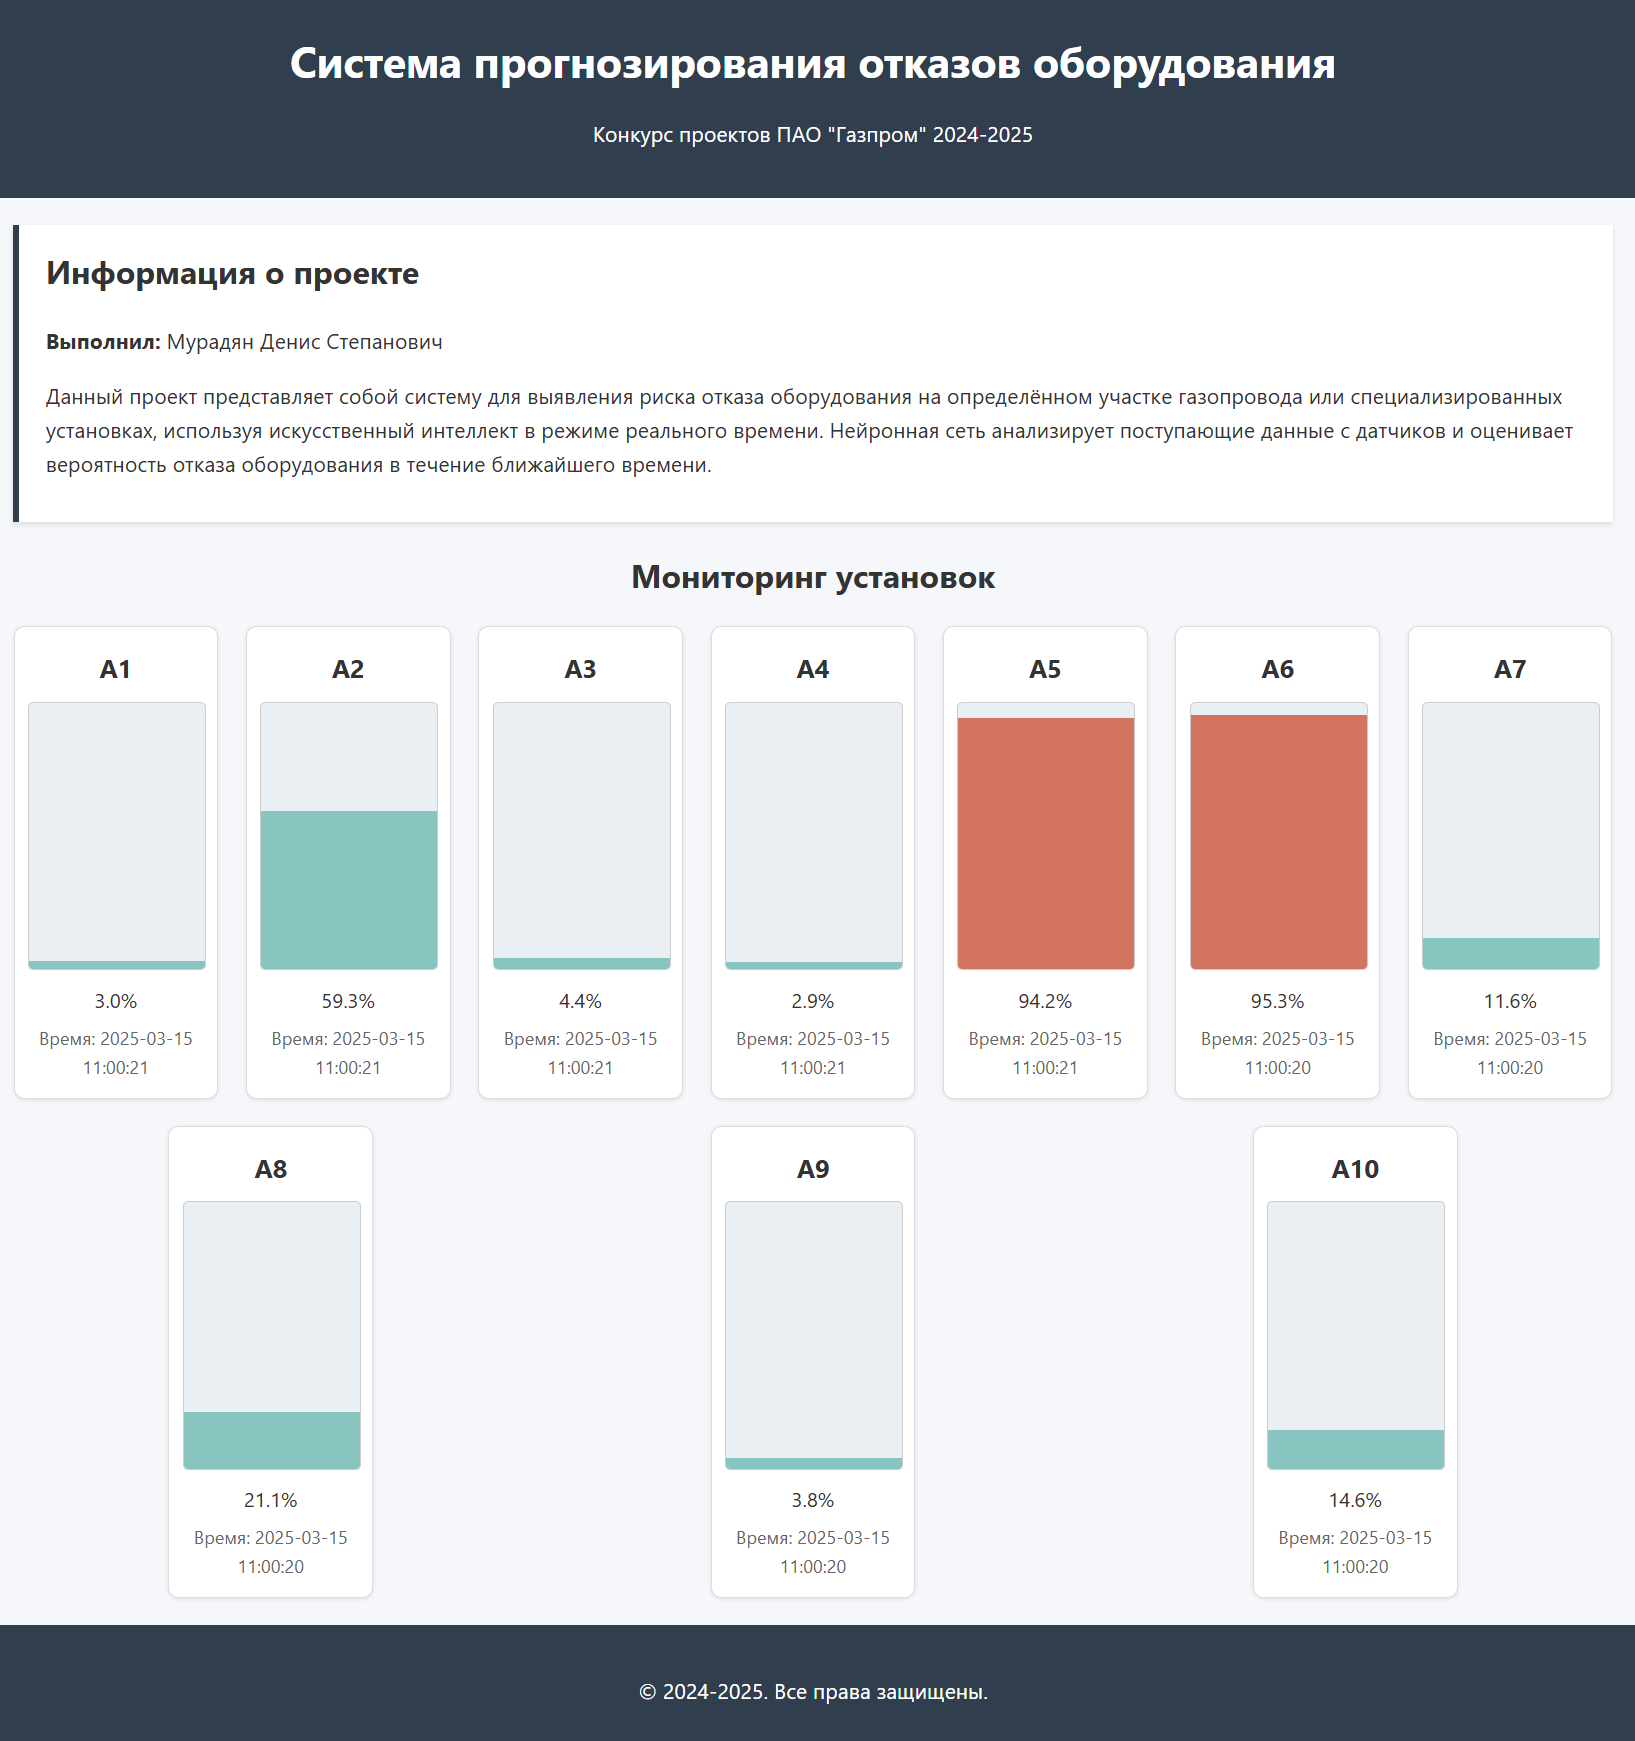
\includegraphics[width=0.6\linewidth]{../../Include/dashboard.png}
\end{frame}

% Слайд 2: Цели проекта
\begin{frame}{Цели проекта}
  \begin{itemize}
    \item Повысить безопасность эксплуатации оборудования за счёт своевременного обнаружения отказов.
    \item Снизить финансовые потери за счёт предотвращения аварийных ситуаций.
    \item Оптимизировать техническое обслуживание с использованием методов искусственного интеллекта.
    \item Интегрировать систему в информационные решения для мониторинга и управления в режиме реального времени.
  \end{itemize}
\end{frame}

% Слайд 3: Новизна проекта
\begin{frame}{Новизна проекта}
  \begin{itemize}
    \item Разработка представляет собой уникальное решение, отличающееся по качеству и масштабируемости от существующих аналогов.
    \item Продукт нового поколения для динамично развивающегося рынка.
    \item Возможность правовой охраны (патентование или регистрация заявки) повышает конкурентоспособность.
  \end{itemize}
\end{frame}

% Слайд 4: Научно-технические особенности
\begin{frame}{Научно-технические особенности}
  \begin{itemize}
    \item \textbf{Использование рекуррентных нейронных сетей:} В основе системы лежит GRU-модель, оптимально учитывающая временные зависимости в последовательностях данных.
    \item \textbf{Обоснование выбора GRU:} В отличие от стандартных RNN, GRU эффективно справляется с проблемой затухания градиента, что позволяет точно прогнозировать редкие аварийные ситуации.
    \item \textbf{Интеграция в систему мониторинга:} Инновационный алгоритм встроен в решение, обеспечивающее анализ данных в режиме реального времени и оперативное реагирование.
  \end{itemize}
\end{frame}

% Слайд 5: Архитектура и компоненты проекта
\begin{frame}{Архитектура и компоненты проекта}
  \begin{columns}
    \column{0.5\textwidth}
      \begin{itemize}
        \item Серверное приложение на FastAPI.
        \item REST API и дашборд для мониторинга в режиме реального времени.
        \item Модули для сбора, обработки данных и предсказания отказов.
      \end{itemize}
    \column{0.5\textwidth}
      \centering
      % Замените placeholder_architecture.png на схематичное изображение архитектуры системы
      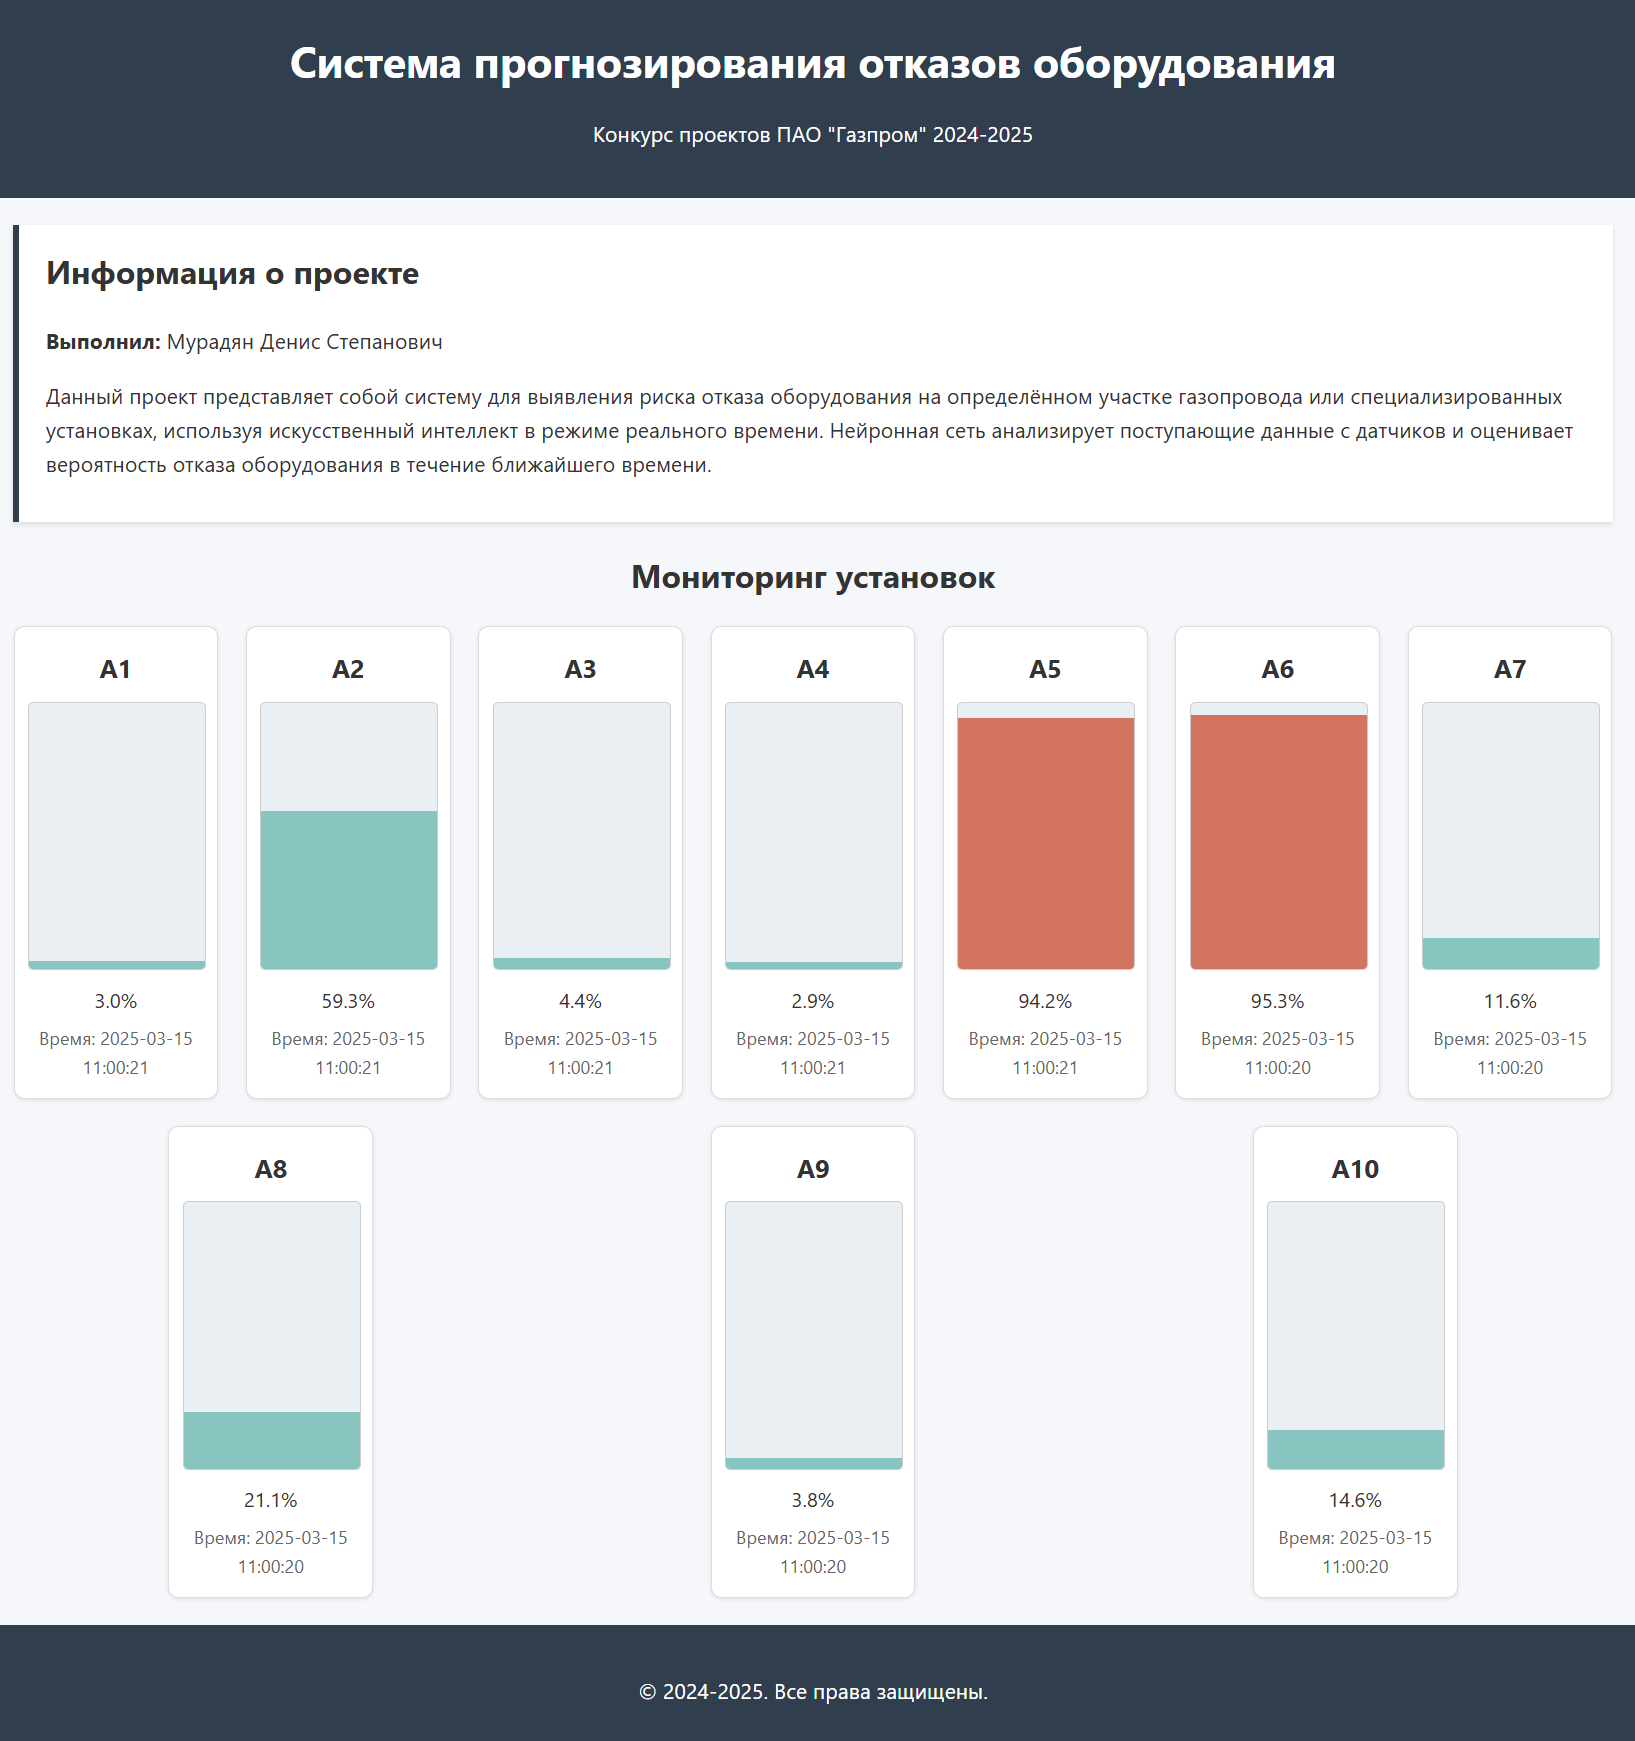
\includegraphics[width=\linewidth]{../../Include/dashboard.png}
  \end{columns}
\end{frame}

% Слайд 6: Методология и обработка данных
\begin{frame}{Методология и обработка данных}
  \begin{itemize}
    \item Генерация синтетического датасета, имитирующего реальные условия работы оборудования.
    \item Нормализация и предварительная обработка данных для корректного анализа временных последовательностей.
    \item Настройка гиперпараметров и логирование процесса обучения модели.
  \end{itemize}
  \vspace{0.3cm}
  \centering
  % Замените placeholder_data.png на иллюстрацию работы с данными
  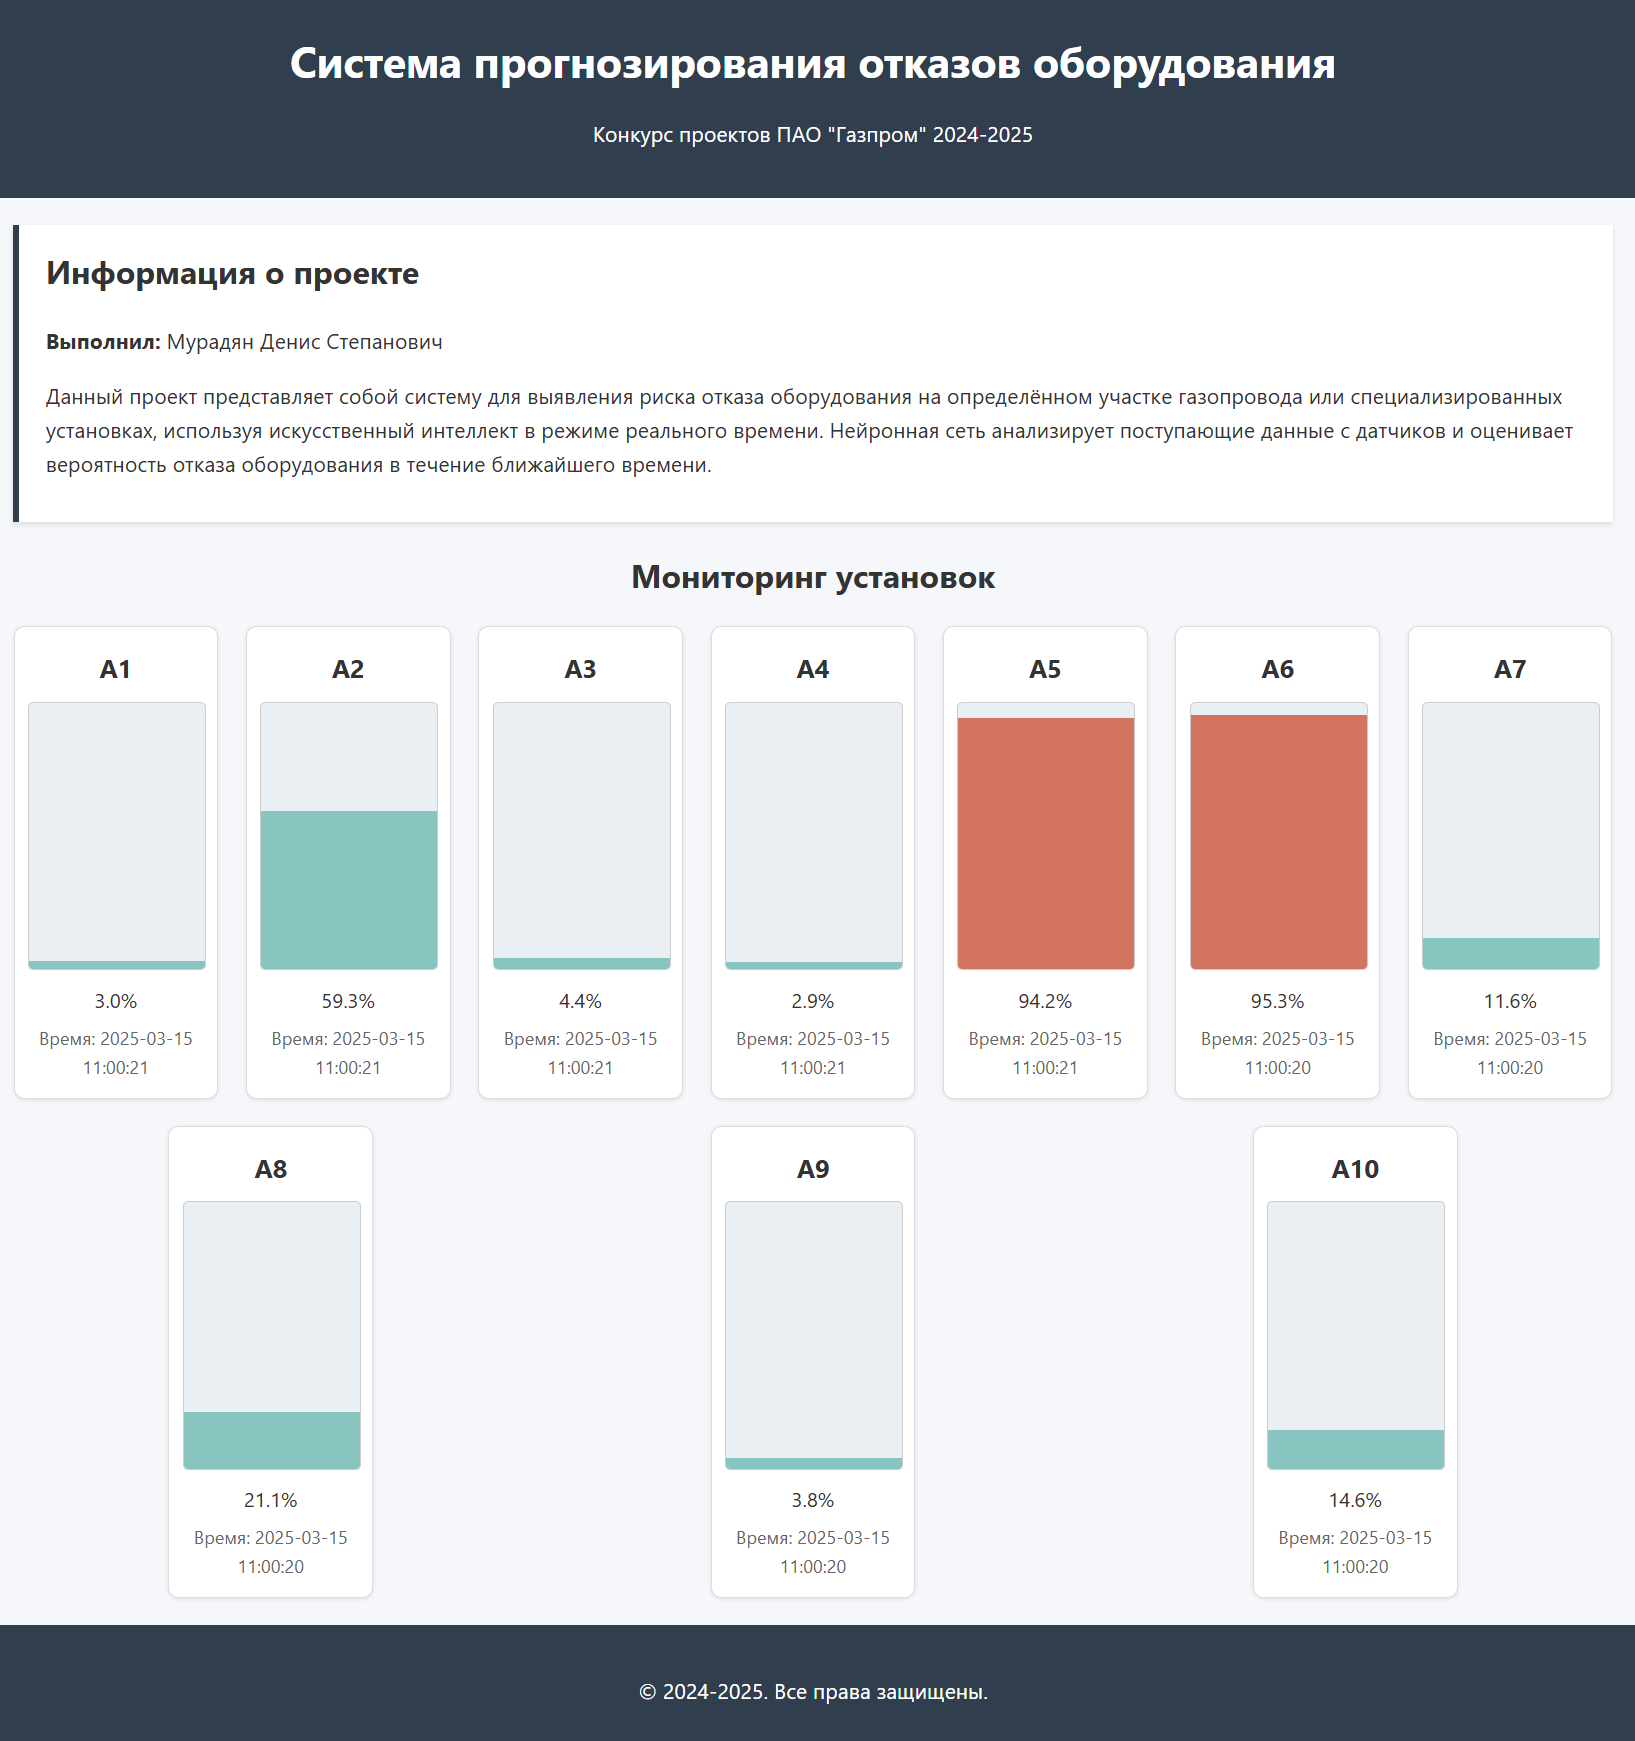
\includegraphics[width=0.5\linewidth]{../../Include/dashboard.png}
\end{frame}

% Слайд 7: Технические результаты и характеристики
\begin{frame}{Технические результаты и характеристики}
  \begin{itemize}
    \item \textbf{Тип модели:} GRU-based RNN.
    \item \textbf{Архитектура:} 2 слоя (64 и 32 нейрона).
    \item \textbf{Функция потерь:} Focal Loss.
    \item \textbf{Метрики:} Accuracy 91.25\%, AUC 0.9777, Precision 84.90\%, Recall 91.78\%.
    \item \textbf{Количество эпох:} 50.
    \item \textbf{Время обучения:} 190.22 секунд.
    \item \textbf{Используемая память:} 512.71 MB.
  \end{itemize}
\end{frame}

% Слайд 8: Готовность и внедрение
\begin{frame}{Готовность и внедрение}
  \begin{itemize}
    \item Система успешно прошла опытную проверку.
    \item Доступ к системе реализован через REST API и онлайн дашборд.
    \item Возможность масштабирования и интеграции в инфраструктуру крупных предприятий.
  \end{itemize}
  \vspace{0.3cm}
  \centering
  % Замените placeholder_ready.png на изображение интерфейса системы
  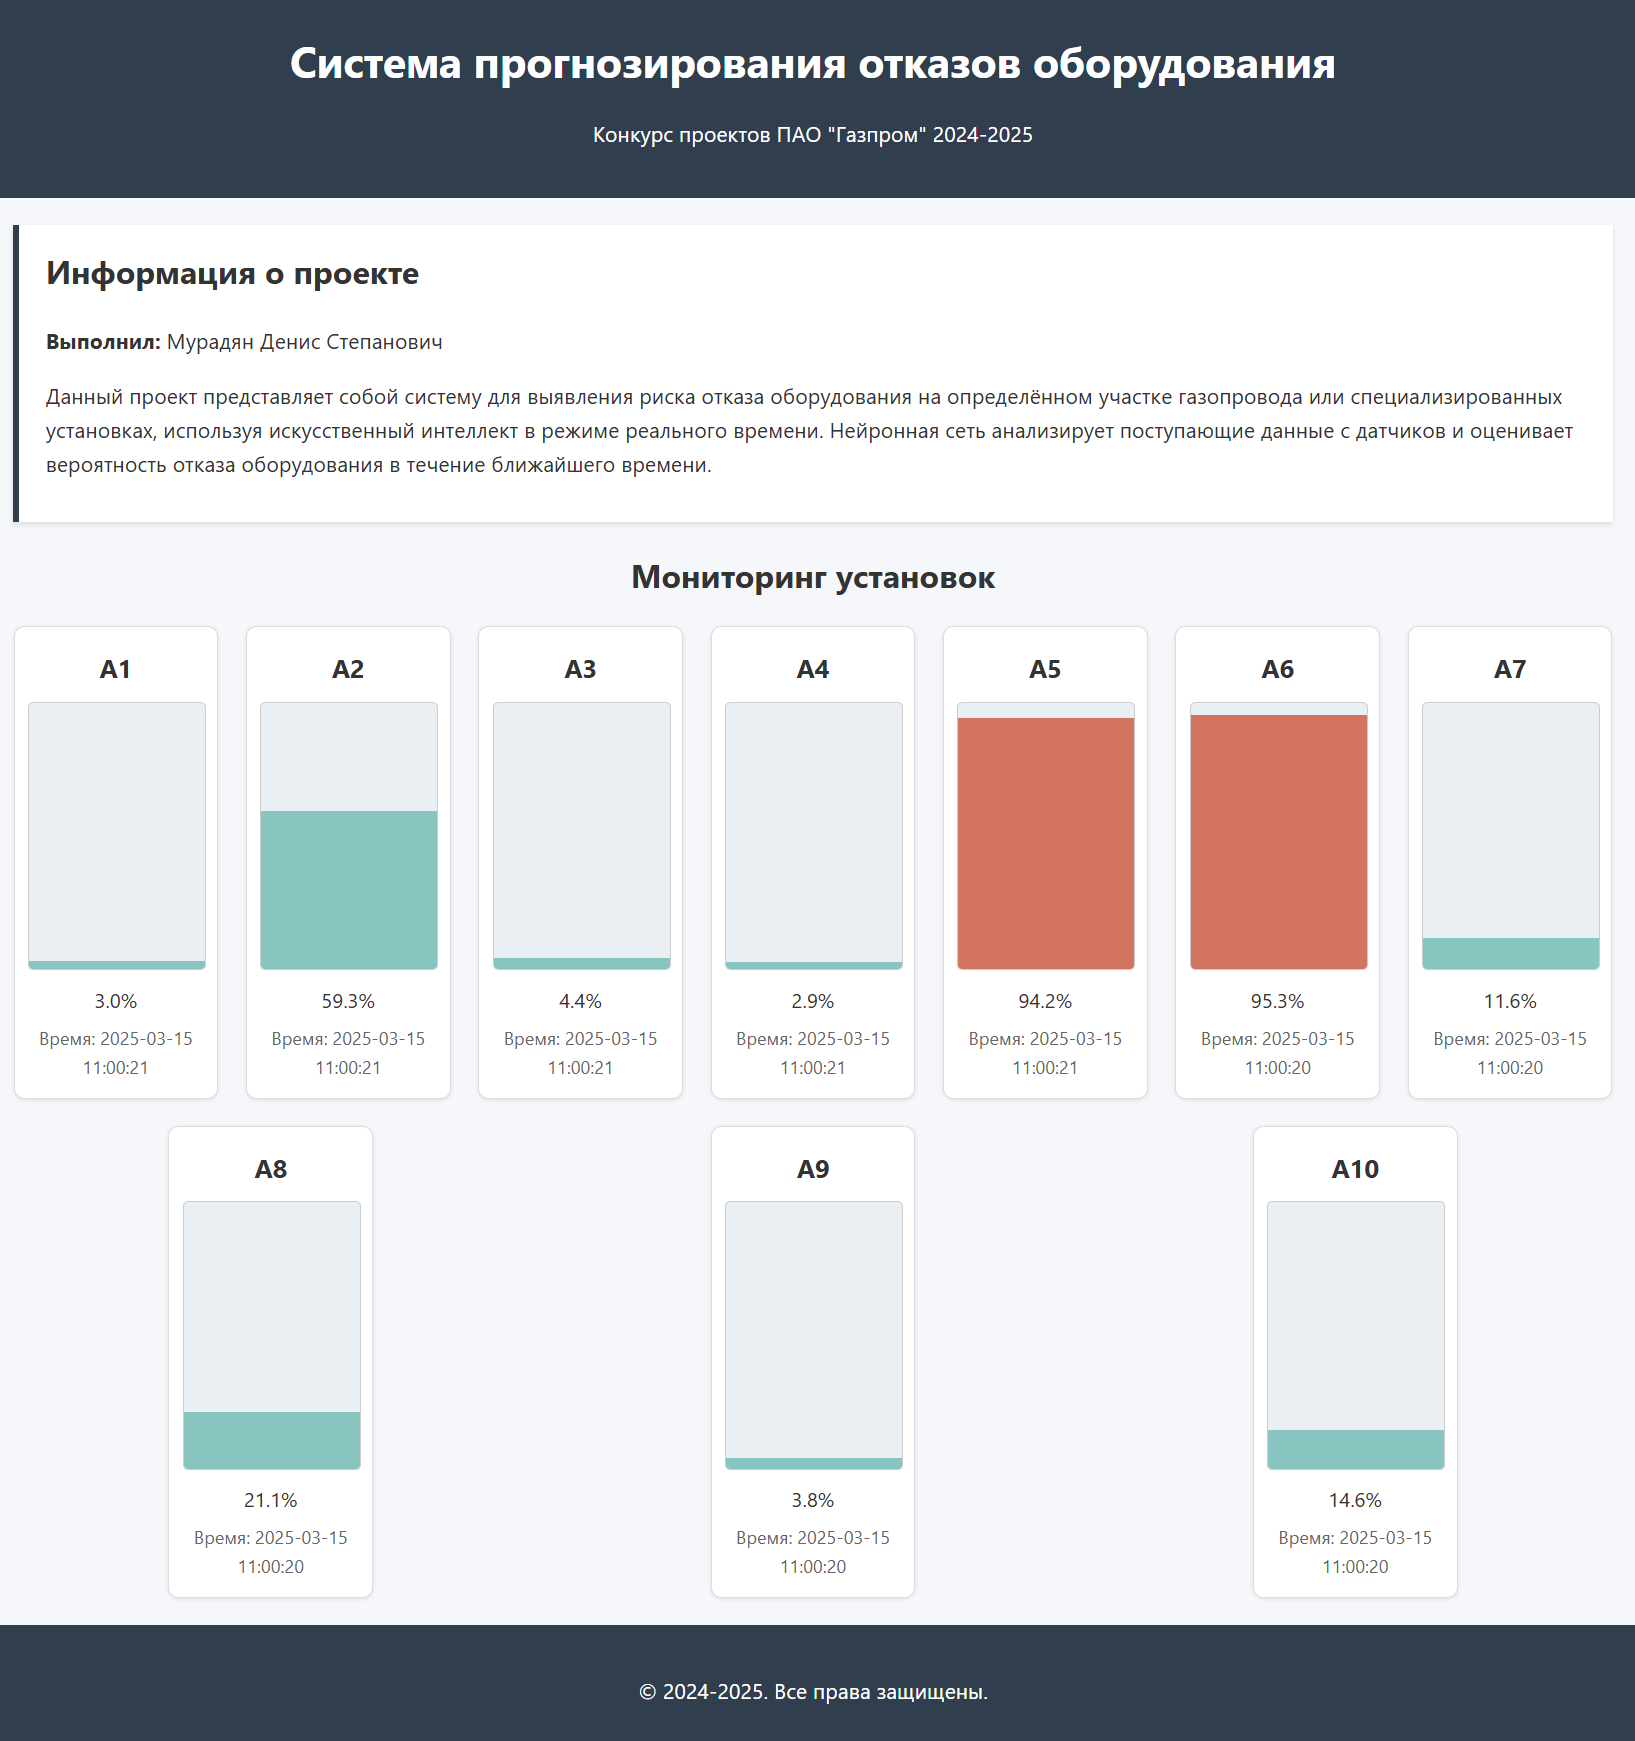
\includegraphics[width=0.5\linewidth]{../../Include/dashboard.png}
\end{frame}

% Слайд 9: Перспективы применения
\begin{frame}{Перспективы применения}
  \begin{itemize}
    \item Широкие возможности коммерциализации в нефтегазовой отрасли.
    \item Применение результатов в образовательном процессе вузов (новые курсы, лабораторные работы).
    \item Подтвержденная заинтересованность потенциальных пользователей и партнеров.
  \end{itemize}
\end{frame}

% Слайд 10: Стратегия реализации и дальнейшее развитие
\begin{frame}{Стратегия реализации и дальнейшее развитие}
  \begin{itemize}
    \item Четкий план продвижения продукта на выбранный сегмент рынка.
    \item Дальнейшая инженерная доработка и расширение функционала (например, мобильные оповещения, интеграция с ERP-системами).
    \item Постоянное развитие продукта на основе отзывов пользователей и рыночных трендов.
  \end{itemize}
\end{frame}

% Слайд 11: Заключение и вопросы
\begin{frame}{Заключение и вопросы}
  \begin{block}{Ключевые выводы}
    \begin{itemize}
      \item Проект обеспечивает высокую точность прогнозирования и оперативное реагирование.
      \item Решение соответствует современным требованиям безопасности и экономической эффективности.
      \item Система готова к быстрому внедрению и масштабированию в промышленной среде.
    \end{itemize}
  \end{block}
  \centering
  \Large Вопросы?
\end{frame}

\end{document}
